\capitulo{3}{Conceptos teóricos}

\section{Conceptos teóricos básicos}

En este capítulo se presentan los conceptos teóricos fundamentales que sustentan el desarrollo del sistema de monitoreo cardíaco en tiempo real, permitiendo a cualquier lector comprender el trabajo realizado. Se abordarán temas relacionados con las enfermedades cardiovasculares, la tecnología utilizada, y los métodos de análisis de datos.

\subsection{El Sistema cardiovascular}

El sistema cardiovascular está compuesto por el corazón, los vasos sanguíneos y la sangre. Su función principal es el transporte de oxígeno y nutrientes a los tejidos del cuerpo y la eliminación de desechos metabólicos. El corazón actúa como una bomba que impulsa la sangre a través de los vasos sanguíneos, y la función adecuada de este sistema es crucial para mantener la homeostasis y la salud general del cuerpo \cite{guyton2006text}.

\subsection{Anatomía del Sistema Cardiovascular}

\subsubsection{El corazón}
El corazón es un órgano muscular situado en el mediastino, entre los pulmones. Está compuesto por cuatro cámaras: dos aurículas (derecha e izquierda) y dos ventrículos (derecho e izquierdo). La sangre fluye a través de estas cámaras, siendo impulsada por las contracciones rítmicas del músculo cardíaco. Las paredes del corazón están formadas por tres capas: el endocardio, el miocardio y el pericardio \cite{sistema_cardiovascular}.

\subsubsection{Los vasos sanguíneos}
Existen tres tipos principales de vasos sanguíneos: arterias, venas y capilares. Las arterias transportan la sangre rica en oxígeno desde el corazón hacia los tejidos del cuerpo, mientras que las venas devuelven la sangre pobre en oxígeno al corazón. Los capilares, que son los vasos más pequeños, facilitan el intercambio de oxígeno, nutrientes y desechos entre la sangre y los tejidos \cite{sistema_cardiovascular}.

\subsection{Función del sistema cardiovascular}

El sistema cardiovascular realiza varias funciones esenciales:
\begin{itemize}
    \item \textbf{Transporte de nutrientes y oxígeno:} La sangre transporta oxígeno y nutrientes a las células del cuerpo y elimina dióxido de carbono y otros desechos metabólicos \cite{sistema_cardiovascular}.
    \item \textbf{Regulación de la temperatura corporal:} Mediante la redistribución del flujo sanguíneo, el sistema cardiovascular ayuda a mantener la temperatura corporal \cite{sistema_cardiovascular}.
    \item \textbf{Protección:} La sangre contiene células inmunitarias que defienden al cuerpo contra infecciones y enfermedades \cite{guyton2006text}.
    \item \textbf{Homeostasis:} Mantiene el equilibrio de electrolitos y el pH en el cuerpo, cruciales para el funcionamiento normal de las células \cite{guyton2006text}.
\end{itemize}

\subsection{Enfermedades cardiovasculares}

Las enfermedades cardiovasculares (ECV) son la principal causa de muerte a nivel mundial, representando aproximadamente el 31\% de todas las muertes globales según la Organización Mundial de la Salud (OMS) \cite{who-cvd}. Estas enfermedades incluyen trastornos como la cardiopatía coronaria, la insuficiencia cardíaca, la hipertensión arterial y las arritmias, entre otros. La detección temprana y el monitoreo continuo son cruciales para la prevención y el tratamiento efectivo de estas patologías.

\subsection{Tipos de enfermedades cardiovasculares}

Las enfermedades cardiovasculares corresponden a los trastornos del sistema circulatorio, que incluye el corazón, los vasos sanguíneos y la sangre. Se clasifican en cuatro tipos generales: enfermedades isquémicas del corazón, enfermedades cerebrovasculares, enfermedades vasculares periféricas y otras enfermedades \cite{corella2007enfermedades}.

\subsubsection{Enfermedades isquémicas del corazón}

Estas enfermedades se deben a un estrechamiento progresivo de las arterias coronarias causado por la formación de placas de ateroma. Este engrosamiento de la pared arterial obstruye el flujo sanguíneo, lo que puede provocar isquemia y, si persiste, infarto de miocardio \cite{corella2007enfermedades}.

\subsubsection{Enfermedades cerebrovasculares}

Estas enfermedades se deben a alteraciones en la circulación cerebral. Se clasifican en isquémicas y hemorrágicas. Las isquémicas se producen por una disminución del flujo sanguíneo hacia una región del cerebro, causando infarto cerebral. Las hemorrágicas se deben a la rotura de un vaso sanguíneo en el cerebro \cite{corella2007enfermedades}.

\subsubsection{Enfermedades vasculares periféricas}

Afectan a las arterias o venas que irrigan las extremidades. Provocan dificultades en la circulación sanguínea, estrechamiento de los vasos, hinchazón y dolor. Pueden causar isquemia y, en el caso de las venas, trombosis venosa \cite{corella2007enfermedades}.

\subsubsection{Otras enfermedades cardiovasculares}

Incluyen las cardiopatías congénitas y la cardiopatía reumática. La cardiopatía reumática se produce por infecciones bacterianas que causan lesiones en el miocardio y en las válvulas del corazón \cite{corella2007enfermedades}.

\subsection{Introducción a la monitorización cardíaca}

La monitorización cardíaca es una técnica utilizada para observar y registrar la actividad eléctrica del corazón a lo largo del tiempo. Esta práctica es esencial para la detección de diversas condiciones cardíacas, incluyendo arritmias, infartos de miocardio y otras patologías cardíacas. Los dispositivos de monitorización cardíaca pueden ser no invasivos, como los electrocardiogramas (ECG) tradicionales y los monitores Holter, o invasivos, como los dispositivos implantables que registran la actividad cardíaca de forma continua \cite{MayoClinic_monitoring}.

La importancia de la monitorización cardíaca radica en su capacidad para proporcionar datos críticos que ayudan en el diagnóstico temprano, el manejo y el tratamiento de enfermedades cardíacas. Estos datos permiten a los profesionales de la salud tomar decisiones informadas y personalizar los tratamientos para mejorar los resultados de los pacientes \cite{MayoClinic_monitoring}.

\subsection{Electrocardiograma (ECG)}

El electrocardiograma (ECG) es una herramienta diagnóstica utilizada en los hospitales y centros de salud principalmente, que registra la actividad eléctrica del corazón. Con la función de detectar diversas anomalías cardíacas, como por ejemplo arritmias, infartos de miocardio y otros trastornos del ritmo cardíaco. Un ECG típico incluye las ondas P, Q, R, S y T, que representan diferentes fases del ciclo cardíaco. Toda la información a continuación se ha extraído de \cite{azcona2009electrocardiograma}.

\subsubsection{Definición de un electrocardiograma}

El ECG se trata de un estudio de las variaciones del voltaje en relación con el tiempo, esto se ve representado en una gráfica. Se mide la corriente eléctrica que se está desarrollando en el corazón durante un tiempo determinado, en un ECG normal no suele exceder los 30 segundos la duración de la medición.

\subsubsection{El sistema de conducción del corazón}

Para entender bien las razones del por qué y cómo oscilan las líneas del ECG, hay que conocer y entender el sistema de conducción eléctrica del corazón, el cual está formado por el nodo sinoauricular (nodo SA), el nodo auriculoventricular (nodo AV) y el sistema de His-Purkinje, como se puede ver en la Figura (\ref{fig:conduccion_cardiaca}) \cite{enfermeriatop2024}.

\begin{figure}[h]
    \centering
    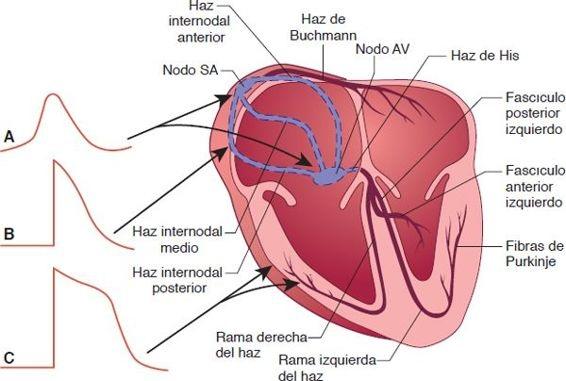
\includegraphics[width=0.6\textwidth]{img/conduccion_cardiaca.png}
    \caption{Sistema de conducción del corazón \cite{enfermeriatop2024}.}
    \label{fig:conduccion_cardiaca}
\end{figure}

\paragraph{Nodo sinoauricular (SA)}
Esta estructura tiene una forma de semiluna y se encuentra localizada detrás de la aurícula derecha, es el lugar donde se inicia el impulso eléctrico del corazón.

\paragraph{Nodo auriculoventricular (AV)}
Se encuentra en la unión entre aurículas y ventrículos, en cuanto al tamaño es la mitad que el del nodo SA. En este caso, el nodo AV tiene como función que las aurículas se contraigan y vacíen su contenido de sangre en los ventrículos antes de producirse la contracción ventricular.

\paragraph{Sistema de His-Purkinje}
El impulso cardíaco se propaga por el haz de His y sus ramas a lo largo del tabique interventricular y se distribuye por toda la masa ventricular a través de las fibras de Purkinje, provocando la contracción de los ventrículos.

\subsection{Interpretación de un electrocardiograma}

El ECG presenta como línea guía la denominada línea isoeléctrica o línea basal. Los latidos cardíacos quedan representados en el ECG por las diferentes oscilaciones de la línea basal en forma de ángulos, segmentos, ondas e intervalos.

\begin{figure}[h]
    \centering
    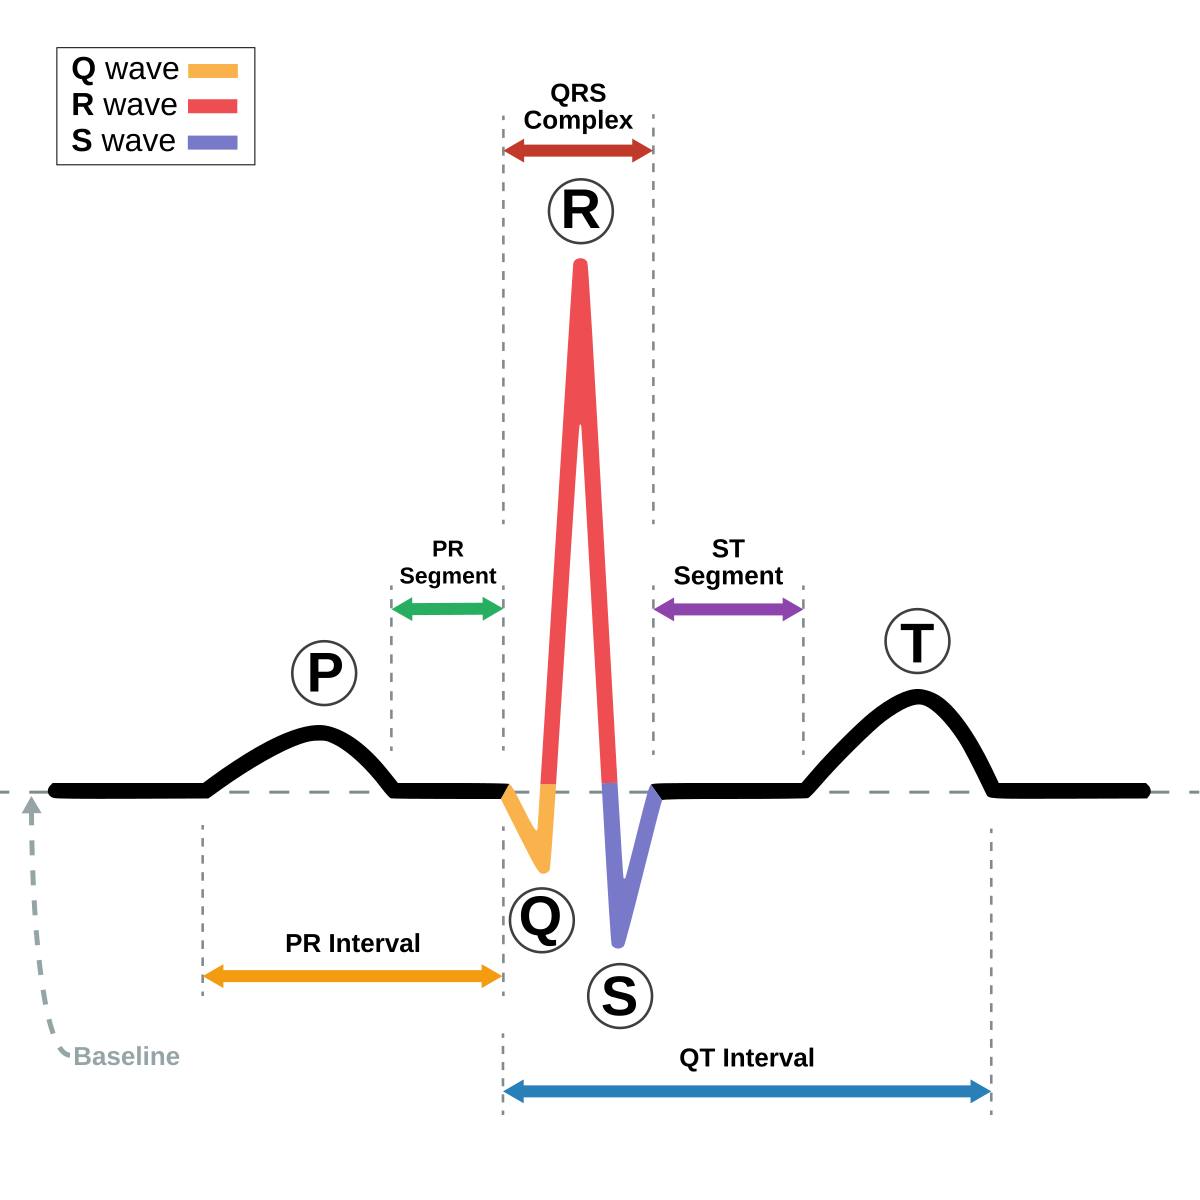
\includegraphics[width=0.5\textwidth]{img/ecg_wave.png}
    \caption{Onda típica del ECG \cite{wikipedia-ecg}.}
    \label{fig:ecg_wave}
\end{figure}

\subsubsection{Onda P}
Es la primera elevación de la onda que aparece en el ECG. Es el momento en que las aurículas se están contrayendo y enviando sangre hacia los ventrículos. Suele durar unos 0.08 segundos.

\subsubsection{Segmento PR}
Es el tramo que aparece entre el final de la onda P y el inicio del complejo QRS. Es el tiempo que tarda el impulso eléctrico en pasar a través del nodo AV.

\subsubsection{Intervalo PR}
El intervalo PR es el período desde el inicio de la onda P hasta el inicio del complejo QRS. Es el tiempo total de conducción auriculoventricular, es decir, el tiempo que tarda el impulso eléctrico en viajar desde el nodo SA, pasando por el nodo AV, hasta el inicio de la despolarización ventricular. Suele durar entre 0.12 y 0.20 segundos \cite{azcona2009electrocardiograma}.

\subsubsection{Complejo QRS}
Es el momento en que los ventrículos se contraen y expulsan su contenido sanguíneo. Consta de las ondas Q, R y S. El complejo QRS no debe exceder en duración más de 0.08 segundos.

\subsubsection{Segmento ST}
Es el trazado de la línea basal entre el final de la onda S y el comienzo de la onda T. Dependiendo de que sufra una elevación o descenso puede indicar insuficiencia en el riego del corazón.

\subsubsection{Onda T}
Sucede después del segmento ST. Es el momento en que el corazón se encuentra en un período de relajación, una vez que ha expulsado la sangre de los ventrículos.

\subsubsection{Intervalo QT}
El intervalo QT se extiende desde el inicio del complejo QRS hasta el final de la onda T. Representa el tiempo total que tarda el músculo ventricular en despolarizarse y repolarizarse. La duración del intervalo QT varía con la frecuencia cardíaca, pero generalmente dura entre 0.36 y 0.44 segundos \cite{azcona2009electrocardiograma}.

\subsection{Importancia de un electrocardiograma}

Realizar un ECG es un procedimiento sencillo que requiere de un electrocardiógrafo, parches de ECG y un sistema de cables. El paciente se coloca boca arriba y se le colocan los parches, cuatro en las extremidades y seis en puntos específicos del pecho, formando así 12 derivaciones.

Los objetivos del ECG principalmente para detectar trastornos del ritmo cardíaco (arritmias) y en el diagnóstico de situaciones con aporte insuficiente de sangre al corazón (infarto de miocardio y angina de pecho).

La importancia del monitoreo continuo reside en la detección temprana de enfermedades cardiovasculares y otras anomalías del ritmo cardíaco, como arritmias. La electrocardiografía (ECG) es una técnica ampliamente utilizada para registrar la actividad eléctrica del corazón. Los datos de ECG permiten a los médicos diagnosticar diversas afecciones cardíacas, desde arritmias hasta enfermedades coronarias. Un ECG típico mide la actividad eléctrica en diferentes puntos del tiempo, proporcionando información sobre el ritmo y la fuerza de los latidos del corazón \cite{MayoClinic_monitoring}.

\subsection{Tecnologías de comunicación}

El sistema de monitoreo utiliza una conexión serial a través del puerto USB para transmitir datos del Arduino a la aplicación web. Este método de comunicación es sencillo y efectivo, lo ideal sería conexión inalámbrica mediante Wi-Fi o Bluetooth pero mirando el lado positivo, realizando la conexión mediante USB para la transmisión de los datos se está eliminando la necesidad de baterías y otra serie de problemas que aparecen en módulos inalámbricos como el HC-05.

\subsection{Comunicación serial}

La comunicación serial permite la transmisión de datos entre el Arduino y la aplicación web a través de un cable USB. Es una forma confiable y directa de transferir grandes volúmenes de datos en tiempo real.

La comunicación serial en Arduino es fundamental para la interacción entre el microcontrolador y dispositivos externos. Utilizando esta comunicación, el Arduino puede enviar y recibir datos en tiempo real, lo que es ideal para proyectos que requieren interacción con sensores, displays u otros componentes de hardware \cite{TechZero2024}.

La configuración de la comunicación serial comienza con la inicialización de la misma mediante la función \texttt{Serial.begin(baudRate)} en el sketch de Arduino. El parámetro \texttt{baudRate} establece la velocidad de transmisión de datos, que debe coincidir en ambos extremos de la comunicación para evitar errores \cite{DeepBluEmbedded2024}.

La comunicación serial es eficiente y ligera en comparación con otras formas de transmisión de datos, proporcionando un control preciso sobre el flujo de información y asegurando una transmisión precisa sin demoras ni errores significativos \cite{TechZero2024}.

Para proyectos que requieren el envío de datos en tiempo real a una aplicación web, la comunicación serial a través de USB ofrece una solución simple y efectiva, facilitando la creación de sistemas de monitoreo interactivos y de alta fiabilidad.

\subsection{Sensor AD8232 y su funcionamiento}

El sensor AD8232 es un módulo especializado en la captación de señales cardíacas, comúnmente utilizado para la creación de electrocardiogramas (ECG). Este sensor es altamente eficiente para detectar la actividad eléctrica del corazón, proporcionando una solución precisa y económica para proyectos de monitoreo cardíaco.

\textbf{Características del sensor AD8232}

El AD8232 destaca por varias características clave que lo hacen ideal para aplicaciones de monitoreo de salud. Entre ellas se encuentran su alta precisión para filtrar y amplificar las señales bioeléctricas del corazón, eliminando el ruido y las interferencias \cite{AD8232_teoria}. Además, el sensor tiene un bajo consumo de energía, lo que lo hace perfecto para dispositivos portátiles \cite{SparkFun_AD8232}. También es fácil de integrar con diversas plataformas de microcontroladores, como Arduino, facilitando su implementación en proyectos de monitoreo cardíaco \cite{liaw2002classification}.

\textbf{Funcionamiento del sensor AD8232}

El sensor AD8232 capta las señales eléctricas del corazón a través de electrodos colocados en la piel del paciente. Estas señales son amplificadas y filtradas para eliminar el ruido y las interferencias, proporcionando una salida analógica que puede ser leída y procesada por un microcontrolador, como una placa Arduino. La señal resultante es una representación precisa de la actividad eléctrica del corazón, similar a un ECG, que puede ser utilizada para monitorear y analizar el ritmo cardíaco en tiempo real \cite{Kumar2020_LowCostECG}.

\textbf{Descripción detallada del sensor AD8232}

El sensor AD8232 incluye varios componentes principales: los electrodos, el amplificador AD8232, los filtros y las salidas. Los electrodos detectan la actividad eléctrica del corazón, que es amplificada por el AD8232. Los filtros incorporados eliminan el ruido, dejando una señal clara del ECG que puede ser visualizada y analizada en tiempo real \cite{AD8232_teoria}.

\textbf{Proceso de medición}

El proceso de medición con el AD8232 incluye la correcta colocación de los electrodos en el cuerpo: RA (Brazo Derecho), LA (Brazo Izquierdo) y RL (Pierna Derecha). Los electrodos detectan las señales eléctricas generadas por la actividad del corazón, que son amplificadas y filtradas por el AD8232. La señal amplificada se envía a un microcontrolador o dispositivo de grabación a través de la salida analógica, donde puede ser visualizada y analizada en tiempo real \cite{SparkFun_AD8232}.

\textbf{Conexiones del sensor AD8232}

El AD8232 tiene varias conexiones importantes: la salida analógica (OUT) se conecta a una entrada analógica de un microcontrolador, los pines de alimentación (3.3V/5V y GND) se conectan a una fuente de alimentación adecuada, y los pines de electrodo (RA, LA, RL) se conectan a los respectivos electrodos en el cuerpo \cite{AD8232_teoria}.


\subsection{Desarrollo web}

Para el desarrollo de la aplicación web se usan las tecnologías frontend y backend que colaboran para darnos una interfaz intuitiva y funcional. Es clave entender las diferencias y las interacciones entre el frontend y el backend para crear un software efectivo \cite{PrimeIT}.

\subsubsection{Frontend}

El frontend de la aplicación web ha sido desarrollado con el framework Streamlit, que permite la creación rápida de interfaces interactivas en Python. Streamlit facilita la visualización de datos en tiempo real y proporciona una experiencia de usuario fluida. El frontend es el diseño y desarrollo de la interfaz de usuario, aspectos como la accesibilidad, la estructura de navegación, la capacidad de respuesta y las animaciones. Se utilizan lenguajes como CSS, HTML y JavaScript \cite{PrimeIT}. Esta enfocado en la experiencia del usuario, asegurando que la interfaz sea intuitiva y atractiva.

\subsubsection{Backend}

El backend, también desarrollado en Python, se encarga del procesamiento de datos y la gestión de la base de datos SQLite. Esta base de datos almacena las predicciones realizadas por el modelo de machine learning. El backend es la parte de la funcionalidad, que se encarga de gestionar los recursos, implementando la lógica del sistema e integrando los servidores web y bases de datos. Entre los lenguajes de programación comúnmente utilizados en el backend se incluyen Java, Python y PHP \cite{PrimeIT}.

\subsection{Desarrollo de la base de datos}

Para almacenar todos los datos obtenidos durante la predicción de clases de ciclos cardiacos del paciente, es necesario diseñar una base de datos adecuada. El diseño de bases de datos implica decidir su propósito y organizar la información por temas. Cada tabla debe tener claves únicas que identifiquen cada fila de manera individual y definir cómo se relacionan entre sí. Existen dos tipos principales de bases de datos:


\subsubsection{Bases de datos relacionales}

Este tipo de base de datos se busca mantener la máxima integridad y precisión de la información, lo cual puede causar una mayor lentitud por que se realiza el procesamiento de los datos antes que el almacenamiento. Está diseñada para garantizar la exactitud y consistencia de los datos, priorizando la eficiencia y veracidad sobre la velocidad. Ejemplos de bases de datos relacionales son PostgreSQL y MySQL \cite{Structuralia}. En este proyecto, se ha utilizado SQLite, una base de datos relacional.

\subsubsection{Bases de datos no relacionales}

Por otro lado, las bases de datos no relacionales buscan el almacenamiento rápido de los datos sobre la exactitud, reduciendo las restricciones y, a veces, sacrificando la veracidad. El análisis de los datos se realiza posteriormente. Este tipo de base de datos es adecuado cuando la velocidad es crucial y la estructura de los datos puede ser más flexible. Firebase es un ejemplo de una base de datos no relacional \cite{Structuralia}.

\subsection{Visualización y grabación de datos}

El sistema cuenta con una aplicación desarrollada en Tkinter, que permite la visualización y grabación de los datos de ECG en tiempo real. Tkinter es una biblioteca de interfaces gráficas para Python que facilita la creación de ventanas y elementos interactivos \cite{tkinter_docs}.

Para la visualización de datos en tiempo real, Tkinter utiliza su función de actualización periódica que permite refrescar la interfaz con nuevos datos continuamente. Esto es esencial en aplicaciones de monitoreo como el ECG, donde es crucial visualizar las señales cardíacas a medida que se generan \cite{tkinter_real_time}.

La integración de Tkinter con bibliotecas de visualización de gráficos como Matplotlib permite representar los datos de ECG en gráficos dinámicos. Matplotlib facilita la creación de gráficos en 2D que se pueden integrar fácilmente en las ventanas de Tkinter, proporcionando una visualización clara y en tiempo real de los datos de ECG \cite{matplotlib}.

La grabación de datos en Tkinter se puede manejar mediante la captura de datos en intervalos regulares y su almacenamiento en archivos o bases de datos. Esto es útil para realizar análisis posteriores o para mantener un registro histórico de las señales de ECG para su revisión \cite{tkinter_data_logging}.

En resumen, la combinación de Tkinter y Matplotlib proporciona una plataforma poderosa y flexible para la visualización y grabación de datos en tiempo real en aplicaciones médicas, como el monitoreo cardíaco, ofreciendo una interfaz intuitiva y funcional para los usuarios \cite{tkinter_matplotlib_integration}.

\subsection{Modelo de predicción}

Se ha utilizado un modelo de Random Forest, este modelo ha sido entrenado con datos de ECG obtenidos de Kaggle \cite{kaggle-data}, que incluyen etiquetas como Latidos Normales, Latidos de Ectopia Supraventricular, Latidos de Ectopia Ventricular, Latidos de Fusión y Latidos Inclasificables.

El modelo de predicción basado en Random Forest es una técnica de aprendizaje automático utilizada tanto para problemas de clasificación como de regresión. Es conocido por su alta precisión, capacidad de manejar grandes conjuntos de datos y su resistencia al sobreajuste (overfitting). A continuación, se presenta una explicación teórica detallada del modelo Random Forest, junto con referencias bibliográficas para una comprensión más profunda \cite{randomforest-medium}.

El Random Forest es un conjunto de árboles de decisión entrenados de manera individual en diferentes subconjuntos del conjunto de datos. Cada árbol vota por una clase y la clase con más votos se selecciona como la predicción final. Este enfoque reduce el riesgo de sobreajuste y mejora la precisión del modelo al promediar los resultados de múltiples árboles. Random Forest también proporciona una medida de importancia de las características, lo que puede ser útil para entender cuáles son las características más relevantes para la predicción \cite{randomforest-medium}.

La Figura \ref{fig:RandomForest} muestra un diagrama del modelo Random Forest utilizado para la predicción de latidos cardíacos.

\begin{figure}[h]
\centering
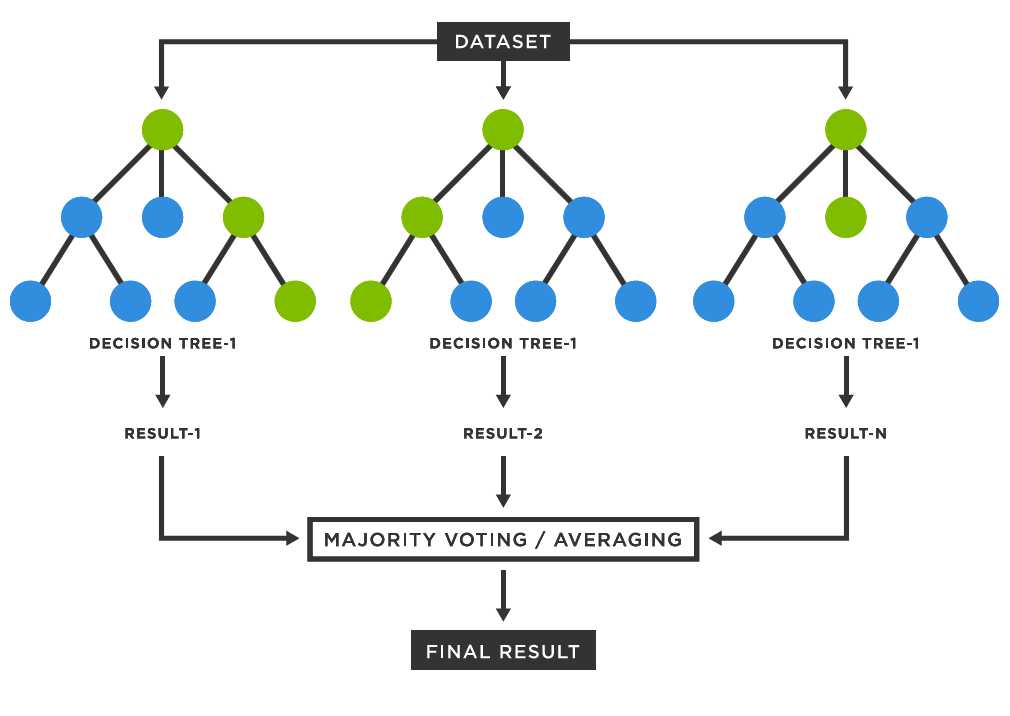
\includegraphics[width=0.5\textwidth]{img/randomforest.png}
\caption{Diagrama del modelo Random Forest utilizado para la predicción de latidos cardíacos \cite{randomforest-medium}.}
\label{fig:RandomForest}
\end{figure}

\subsection{Fundamentos del random forest}

Random Forest es un algoritmo de aprendizaje de conjunto (ensemble learning) que combina múltiples árboles de decisión para mejorar la precisión y robustez del modelo. Un árbol de decisión es una estructura de datos en forma de árbol donde cada nodo interno representa una "prueba" en una característica, cada rama representa el resultado de la prueba, y cada hoja representa una etiqueta de clase (en clasificación) o un valor continuo (en regresión) \cite{breiman2001random}. Random Forest utiliza el método de Bootstrap Aggregating (Bagging), que genera múltiples subconjuntos del conjunto de datos original mediante muestreo con reemplazo. Cada subconjunto se utiliza para entrenar un árbol de decisión independiente, reduciendo la varianza del modelo y mejorando la estabilidad y precisión \cite{breiman1996bagging}. Además, para cada nodo en un árbol de decisión, Random Forest selecciona aleatoriamente un subconjunto de características y elige la mejor división basada en estas características, lo cual reduce la correlación entre los árboles individuales y mejora la precisión del modelo. Una vez que todos los árboles han sido entrenados, el resultado final de Random Forest se obtiene mediante la agregación de las predicciones de todos los árboles. En problemas de clasificación, se utiliza la votación mayoritaria, mientras que en problemas de regresión se calcula el promedio de las predicciones \cite{breiman2001random}.

Se emplea un modelo de machine learning basado en Random Forest para realizar predicciones sobre los segmentos de ECG. Este modelo ha sido entrenado utilizando datos de Kaggle \cite{kaggle-data}, y es capaz de clasificar diferentes tipos de latidos cardíacos.

\subsection{Preparación de los datos}

Los datos de ECG se preprocesaron para extraer características relevantes que el modelo pudiera utilizar para la predicción. Este proceso incluyó la normalización de los datos y la segmentación de los ciclos cardíacos. Cada segmento del ECG se etiquetó con el tipo de latido correspondiente.

\subsubsection{Detección de picos R}

La detección de picos R es crucial para identificar los latidos del corazón en los datos de ECG. Se utiliza la función \texttt{find\_peaks} de Scipy para localizar estos picos.

\subsubsection{Segmentación de latidos}

Los segmentos de latidos se extraen centrados en los picos R detectados. Cada segmento incluye una cantidad fija de muestras antes y después del pico R para capturar un ciclo cardíaco completo y se rellena con valores 0 hasta que alcanza las 187 muestras, esto ocurre porque tiene que ser de la misma longitud que los datos de entrenamiento y test, los cuales cada segmento que corresponde a un latido está conformado por 187 muestras.

\subsection{Entrenamiento del modelo}

El modelo de Random Forest se entrenó utilizando el conjunto de datos preprocesados. Se utilizó una validación cruzada para evaluar el rendimiento del modelo y ajustar los parámetros para mejorar su precisión. El modelo final se guardó utilizando la biblioteca \texttt{Joblib} para su posterior uso en la aplicación web.

\subsection{Implementación en la aplicación web}

El modelo de predicción se integró en el backend de la aplicación web desarrollada con Streamlit. Cuando los datos de ECG se reciben en la aplicación, se procesan y segmentan en tiempo real. Cada segmento se pasa al modelo de Random Forest, que predice el tipo de latido. Los resultados se muestran en la interfaz de usuario y se pueden almacenar en la base de datos para su posterior análisis.

\subsection{Elección del modelo predictivo: Random Forest}

La elección del modelo de predicción es una decisión muy importante en el desarrollo de cualquier sistema de aprendizaje automático. En este proyecto, se ha optado por utilizar el modelo Random Forest para la clasificación de latidos cardíacos por las razones que se van a explicar y demostrar a continuación.

\subsubsection{Ventajas del Random Forest}

El modelo Random Forest se ha elegido por varias razones clave, que se detallan a continuación:

\begin{itemize}
\item \textbf{Robustez y estabilidad:} Random Forest es un modelo de ensamblaje que combina múltiples árboles de decisión, lo que reduce la varianza del modelo y mejora la precisión al evitar el sobreajuste. Evitar el sobreajuste es algo clave de cara a nuestro proyecto ya que va a trabajar todo el rato con datos nuevos y puede que de pacientes diferentes, por lo tanto es esencial para asegurar que el modelo funcione bien con datos nuevos y no vistos \cite{breiman2001random}.
\item \textbf{Manejo de datos faltantes y no lineales:} Una de las principales ventajas de Random Forest es su capacidad para manejar datos faltantes y capturar relaciones no lineales en los datos. Esto es especialmente útil en aplicaciones médicas donde los datos pueden estar incompletos o presentar relaciones complejas \cite{ho1995random}.
\item \textbf{Facilidad de uso e implementación:} Random Forest requiere menos ajuste de parámetros en comparación con otros modelos complejos como las redes neuronales. Además, su implementación es sencilla utilizando bibliotecas como scikit-learn en Python, lo que facilita su uso en diferentes aplicaciones \cite{scikit-learn}.
\item \textbf{Interpretabilidad:} A diferencia de otros modelos de caja negra, Random Forest permite a los desarrolladores entender qué características son más influyentes en las predicciones \cite{liaw2002classification}.
\end{itemize}

\subsubsection{Comparación con otros modelos}

Aunque otros modelos como las redes neuronales artificiales (ANN), K-Nearest Neighbors (KNN), Support Vector Machine (SVM), Gradient Boosting y Decision Trees también son efectivos, Random Forest ofrece una combinación única de características que lo hacen ideal para este proyecto y a continuación se va a realizar una comparación con otros modelos usando en todos ellos los mismos conjuntos de datos de entrenamiento y de test, los resultados obtenidos aparecen en la Tabla \ref{tab:comparison}.

\begin{itemize}
\item \textbf{ANN:} Las ANN pueden ofrecer un rendimiento ligeramente superior en términos de métricas, pero requieren más recursos computacionales y tiempo para el entrenamiento. Además, las ANN son menos interpretables que Random Forest \cite{goodfellow2016deep}.
\item \textbf{KNN y SVM:} Aunque son efectivos, estos modelos pueden ser menos escalables y más sensibles a los datos ruidosos en comparación con Random Forest \cite{hastie2009elements}.
\item \textbf{Gradient boosting:} Ofrece un alto rendimiento pero es más complejo de ajustar y entrenar en comparación con Random Forest \cite{friedman2001greedy}.
\item \textbf{Decision tree:} Aunque es sencillo e interpretable, un solo árbol de decisión no es tan robusto ni preciso como un conjunto de árboles como Random Forest \cite{breiman2001random}.
\end{itemize}

\subsubsection{Resultados del modelo Random Forest}

Los resultados obtenidos con el modelo de Random Forest se detallan en la siguiente tabla \ref{tab:comparison}:

\begin{table}[h]
    \centering
    \begin{tabular}{lcccc}
        \toprule
        Modelo & Precisión & F1 Score & Precisión & Recall \\
        \midrule
        Random Forest & 0.9747 & 0.9731 & 0.9748 & 0.9747 \\
        Decision Tree & 0.9527 & 0.9528 & 0.9530 & 0.9527 \\
        SVM & 0.9680 & 0.9657 & 0.9676 & 0.9680 \\
        KNN & 0.9736 & 0.9725 & 0.9727 & 0.9736 \\
        Gradient Boosting & 0.9644 & 0.9621 & 0.9634 & 0.9644 \\
        ANN & 0.9756 & 0.9750 & 0.9751 & 0.9756 \\
        \bottomrule
    \end{tabular}
    \caption{Comparación de métricas de diferentes modelos predictivos con el conjunto de datos de entrenamiento con el mismo conjunto de datos de test para cada modelo}
    \label{tab:comparison}
\end{table}

\subsubsection{Conclusión}

En conclusión, Random Forest se destaca por su combinación de robustez, interpretabilidad, facilidad de uso y capacidad para manejar grandes conjuntos de datos de manera eficiente. Estas características lo hacen especialmente adecuado para la tarea de clasificación de latidos cardíacos en este proyecto, proporcionando un equilibrio óptimo entre rendimiento y practicidad.

\section{Estado del arte y trabajos relacionados}

Para entender mejor la importancia de este proyecto en el campo de las tecnologías médicas, es importante ver qué se ha hecho antes y qué avances tecnológicos existen. Esta revisión bibliográfica examina los desarrollos más recientes y analiza proyectos e investigaciones similares. El objetivo es entender la relevancia y el posible impacto del proyecto, proporcionando una base sólida para su desarrollo y asegurando que esté alineado con las necesidades y desafíos actuales del sector.


\subsection{Revisión de tecnologías}

En los últimos años, las tecnologías de monitoreo cardíaco han avanzado significativamente, permitiendo un monitoreo más preciso y continuo de la actividad cardíaca. A continuación, se revisan algunas de las tecnologías más relevantes:

\subsubsection{Sensores de ECG}

Los sensores de ECG son fundamentales para el monitoreo de la actividad eléctrica del corazón. Estos sensores capturan señales bioeléctricas del corazón, que luego son procesadas y analizadas para detectar irregularidades. Los sensores más avanzados utilizan tecnologías de alto rendimiento para garantizar lecturas precisas y consistentes, incluso en entornos móviles.

\subsubsection{Algoritmos de detección de anomalías}

Los algoritmos de machine learning, como Random Forest, se utilizan para detectar anomalías en los datos de ECG. Estos algoritmos analizan grandes volúmenes de datos y aprenden a identificar patrones asociados con condiciones cardíacas específicas. La implementación de estos algoritmos en dispositivos portátiles mejora la capacidad de monitoreo en tiempo real y la precisión en la detección de eventos cardíacos críticos \cite{breiman2001random}.

\subsubsection{Comunicación inalámbrica}

La comunicación inalámbrica, incluyendo tecnologías como Bluetooth Low Energy (BLE) y Wi-Fi, permite la transmisión de datos de ECG desde dispositivos portátiles a aplicaciones móviles y plataformas web. Esto facilita el monitoreo remoto y continuo de los pacientes, mejorando la accesibilidad y la capacidad de respuesta de los profesionales de la salud \cite{TechZero2024}.

\subsection{Revisión de proyectos similares}


Examinar trabajos anteriores en este campo es clave para poder entender las tendencias y retos actuales. Este estudio nos ayuda a detectar qué falta o necesita mejorar en las investigaciones previas. Al conocer mejor las necesidades de los usuarios, podemos dirigir el nuevo proyecto para que sea más útil y específico.

KardiaMobile es un dispositivo portátil de ECG que permite a los usuarios grabar un electrocardiograma en cualquier lugar y momento. Se conecta a una aplicación móvil, ofreciendo resultados instantáneos y la capacidad de enviar los datos directamente a un profesional de la salud para su análisis. Este dispositivo destaca por su facilidad de uso y portabilidad, lo que facilita el monitoreo continuo de los pacientes \cite{kardiamobile}.

El CheckMe Lite no solo realiza lecturas de ECG, sino que también mide la saturación de oxígeno en sangre (SpO2) y la frecuencia cardíaca. Este dispositivo multifuncional proporciona una amplia gama de datos clínicos, siendo ideal para el monitoreo de la salud en general. Su capacidad para integrar múltiples funciones en un solo dispositivo lo convierte en una herramienta valiosa para el monitoreo en el hogar \cite{checkme}.

El Wellue ER1 es un monitor de ECG portátil que permite realizar un seguimiento de la salud cardíaca a largo plazo. Compatible con smartphones, facilita el almacenamiento y la revisión de datos de ECG a través de aplicaciones móviles, ofreciendo a los usuarios una herramienta poderosa para el monitoreo continuo de su salud cardíaca. Su diseño portátil y su facilidad de uso lo hacen accesible para una amplia gama de usuarios \cite{wellue}.

\subsection{Conclusión}

La revisión del estado del arte y los trabajos relacionados muestra que, aunque existen diversas aplicaciones y dispositivos de monitoreo cardíaco, no todos nos dan una solución integrada de bajo costo y fácil acceso para el monitoreo en tiempo real. Este proyecto se alinea con las necesidades actuales del sector médico al proporcionar una herramienta accesible y efectiva para el monitoreo cardíaco continuo, lo que puede tener un impacto significativo en la prevención y tratamiento de enfermedades cardiovasculares.
































